\begin{plan}
\section{Project Plan}
\subsection{Planned deliverables}
The expected deliverables of the final project are as follows:
\begin{itemize}
  \item A functional library for the modelling and analysis of discrete time temporal networks, including:
  \begin{itemize}
      \item Multiple input handlers.
      \item Graph generation.
      \item Graph creation, modification and storage.
      \item Network analysis (core algorithms, metrics).
      \item Basic network visualization.
  \end{itemize}
  \item Showcase of one or more suitable test case temporal networks.
  \item Successful launch of the library as an open-source project on GitHub.
  \item A clear plan for the future development of the library.
\end{itemize}
\subsection{Timeline}
The project timeline is summarized in a Gantt chart\cite{gantt}.
The chart outlines the work completed and the next steps (week five is the current week of the project).
\begin{figure}[h]
    \centering
    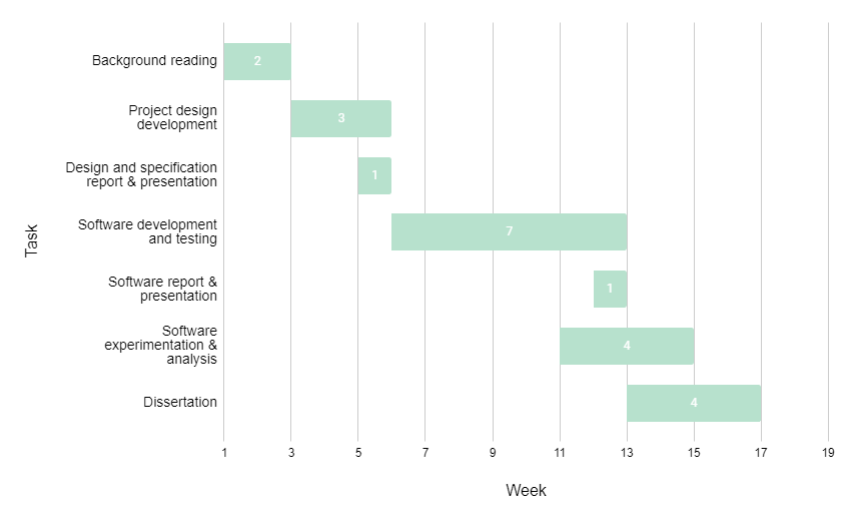
\includegraphics[scale=0.7]{images/timeline.PNG}
    \caption{Project timeline.}
\end{figure}
\clearpage
Figure 12 breaks down 'software development and testing', which is the next major phase of the project for the coming 7 weeks, before the next report is created.
\begin{figure}[h]
    \centering
    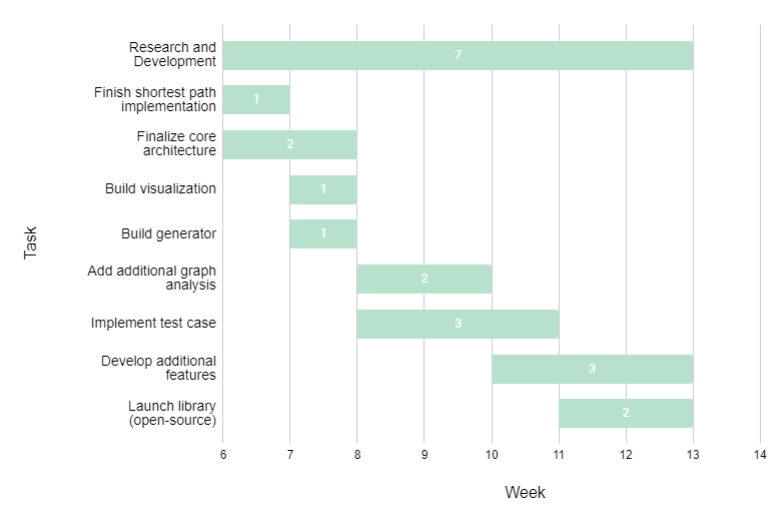
\includegraphics[scale=0.7]{images/dev_timeline.PNG}
    \caption{Software development and testing timeline (weeks 6-12).}
\end{figure}
\end{plan}
\vspace{1cm}
\clearpage